\documentclass[journal,12pt,twocolumn]{IEEEtran}
\usepackage{graphicx}
\graphicspath{{./figs/}}{}
\usepackage{amsmath,amssymb,amsfonts,amsthm}
\newcommand{\myvec}[1]{\ensuremath{\begin{pmatrix}#1\end{pmatrix}}}
\newcommand*{\permcomb}[4][0mu]{{{}^{#3}\mkern#1#2_{#4}}}
\newcommand*{\perm}[1][-3mu]{\permcomb[#1]{P}}
\newcommand*{\comb}[1][-1mu]{\permcomb[#1]{C}}
\usepackage{listings}
\usepackage{watermark}
\usepackage{titlesec}
\let\vec\mathbf
\providecommand{\pr}[1]{\ensuremath{\Pr\left(#1\right)}}
\providecommand{\cbrak}[1]{\ensuremath{\left\{#1\right\}}}
\providecommand{\sbrak}[1]{\ensuremath{{}\left[#1\right]}}
\providecommand{\brak}[1]{\ensuremath{\left(#1\right)}}


\titlespacing{\subsection}{0pt}{\parskip}{-3pt}
\titlespacing{\subsubsection}{0pt}{\parskip}{-\parskip}
\titlespacing{\paragraph}{0pt}{\parskip}{\parskip}
\newcommand{\figuremacro}[5]{
    
}
\lstset{
frame=single, 
breaklines=true,
columns=fullflexible
}
\thiswatermark{\centering \put(0,-105.0){
\includegraphics[scale=0.4]{iith.png}} }

\sloppy
\title{\mytitle}
\title{
Digital Communication Assignment
}
\author{Nikhil Nair}
\begin{document}
\maketitle
%\tableofcontents
\bigskip


\section{\textbf{Problem }}
\begin{enumerate}
\item Generate 
	\begin{align}
		T = U_1+U_2  \nonumber
	\end{align}
\item Find the CDF of $T$.
\item Find the PDF of $T$.
\item Find the theoretical expressions for the PDF and CDF of $T$.
\item Verify your results through a plot. 
\end{enumerate}

\section{\textbf{Solution }}
Let $U1$ and $U2$ are independent uniform random variable between 0 and 1.
\\ 
CDF of $T$ is given as
\begin{align}
F_{T}(x) &= \pr{T \le x}&   \label{eq:1}
\\
&= \pr{U1+U2 \le x}&
\\
F_{T}(x)  &= 
\begin{cases}
0 & 0 < x 
\\
\frac{x^2}{2} & 0 \le x < 1
\\
\frac{-x^2}{2}+2x-1 & 1 < x \le 2 
\\
1 &  x > 2                \label{eq:3}
\end{cases}
\end{align}


The following code generates samples and plots the CDF of $T$.

\begin{lstlisting}
https://github.com/nikhilnair90/FWC/tree/main/Module-II/Digital_Comm/6.4/Code/6_4_cdf.py
\end{lstlisting}

\begin{figure}[h]
    \centering
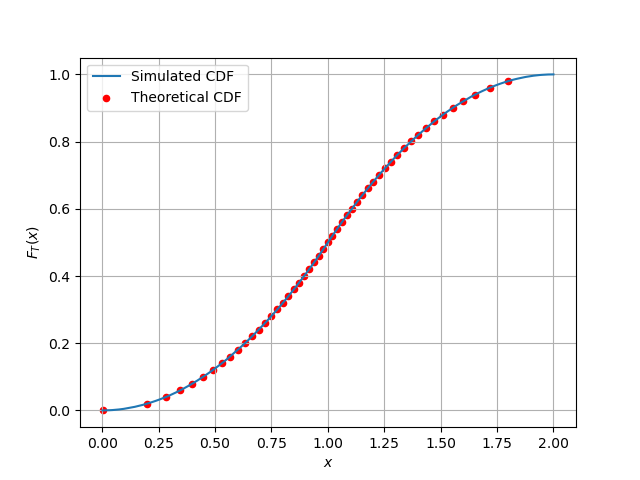
\includegraphics[width=\columnwidth]{figure/cdf.png}
    \label{fig:my_label}
\end{figure}

 
PDF of $T$ is given as
\begin{align}
\pr{T=x}  &= 
\begin{cases}
0 & 0 < x 
\\
x & 0 \le x < 1
\\
2-x & 1 < x \le 2 
\\
1 &  x > 2                \label{eq:4}
\end{cases}
\end{align}
\\
\\
The following code  plots the PDF of $T$.

\begin{lstlisting}
https://github.com/nikhilnair90/FWC/tree/main/Module-II/Digital_Comm/6.4/Code/6_4_pdf.py
\end{lstlisting}

\begin{figure}[h]
    \centering
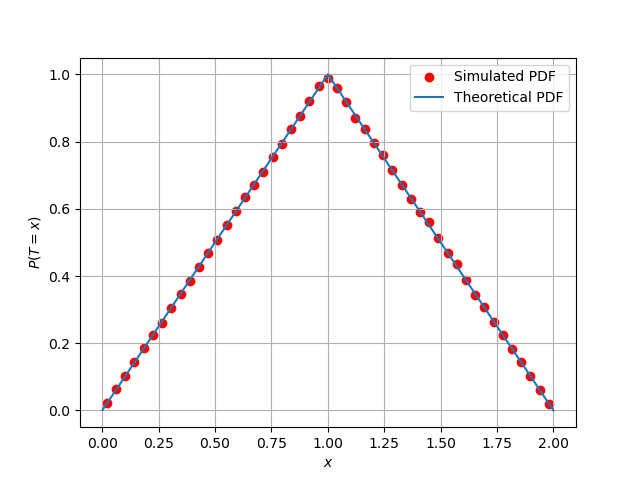
\includegraphics[width=\columnwidth]{figure/pdf.png}
    \label{fig:my_label}
\end{figure}

\end{document}
